One of the most common types of analysis of diffraction data
is to perform an intensity integration in $Q$. This will 
create a plot of average intensity as a function of $Q$.
Since powder diffraction procedures cones of light, this means
that the intensity should be uniformly large for some $Q$
values and uniformly low for others, leading to $Q$ values
where the intensity sharply peaks. The $Q$ values that lead 
to these peaks can be used to learn structural information
about the crystals that are being diffracted. So in principle,
using the transformations just described, it should be easy
to convert all of the pixel coordinates $(x_d,y_d)$ into
$Q$ values and then plot average intensity as a function of
$Q$. The only problem we would face is that in order to do
the transformation, we would need to know the values of the
the parameters that characterize an experiment. These are
\index{$\alpha$}\index{$\beta$}\index{Rotation}
$x_c$, $y_c$, $d$, $\lambda$, $\alpha$, $\beta$, and 
$R$.\footnote{The pixel scale $ps$ is usually know in advance 
as a uniform property of the detector being used.} Calibration
then is the process used to find what we will now call the
calibration values.

\section{The Calibration Algorithm}\label{cal_algorithm}\index{calibration}

Although in principle all the calibration values could be
experimentally measured, in practice they can not be
directly measured to an acceptable level of precision. 
Instead, a standard calibration procedure is used to 
infer these values from real diffraction data. The 
trick to doing this calibration is to image a standard
while performing the diffraction analysis of an 
unknown sample. Assuming that the diffraction machine
was not changed between the collection of the 
standard crystal and the diffraction of the unknown sample, 
the calibration data corresponding to the two 
images will be the same. So, if we can figure out the
calibration values of the standard crystal, we can
use these values when analyzing the unknown crystal.
This is exactly what is done in practice.

What it means to use a standard crystal is to know the
particular $Q$ values for which the crystal preferentially
scatters light. With this information, and the 
calibration values for some particular experiment,
we could in principle figure out exactly what diffraction
pattern we should find. This do this, we could, for
each $Q$ value, vary $\chi$ and calculate the 
$(x_d,y_d)$ coordinate corresponding to that $(Q,\chi)$
pair. After using enough $\chi$ values, we would be 
able to fill in the rings as they would show up on 
the detector.

In fact, my program can do just this. If you load in 
a set of $Q$ values (see section 
\ref{TheQValues})\index{$Q$ Values}
and then put into the program some calibration values,
and then push the \gui{Draw Q Values?} check box, 
you can then see what the particular diffraction
image would have shown up on the detector. 
This is described thoroughly in 
section~\ref{displayconstQlines}

Being able to do this still leaves us with a hard 
problem to solve. For particular calibration values,
we can easily calculate what the diffraction pattern 
should look like. But what we really know is what
the calibration values are for the known diffraction
pattern of a standard crystal. In order to perform the
real calibration, then, we can vary the calibration 
values until they make the pattern that can be calculated
to show up to match the pattern that was actually 
captured. The process of image calibration then is a 
procedure to `fit' the calibration values to a
diffraction patter with known $Q$ values.

\section{The Fitting} 
\index{Fitting}\label{fitting_sec}

In order for the fitting algorithm to work, the program 
must already have an initial guess of the real calibration 
parameters. This initial guess does not have to be perfect, 
but it should be somewhat close. The algorithm them requires 
a list of the known $Q$ values. And it additionally requires 
a range for each of these $Q$ values. In order for the 
algorithm to work properly, inside of this $Q$ range (as 
calculated by the initial calibration value guess) there 
should be the peaks that we are interested in and no spurious 
other peaks that would confuse the computer.

With the $Q$ values specified along with $Q$ ranges, we can
divided up any diffraction image several regions, where
within each region we know there is a unique peak.
An example of this is shown in figure~\ref{divide_up_image}.

\begin{SCfigure}[1][htbp]
    \centering
    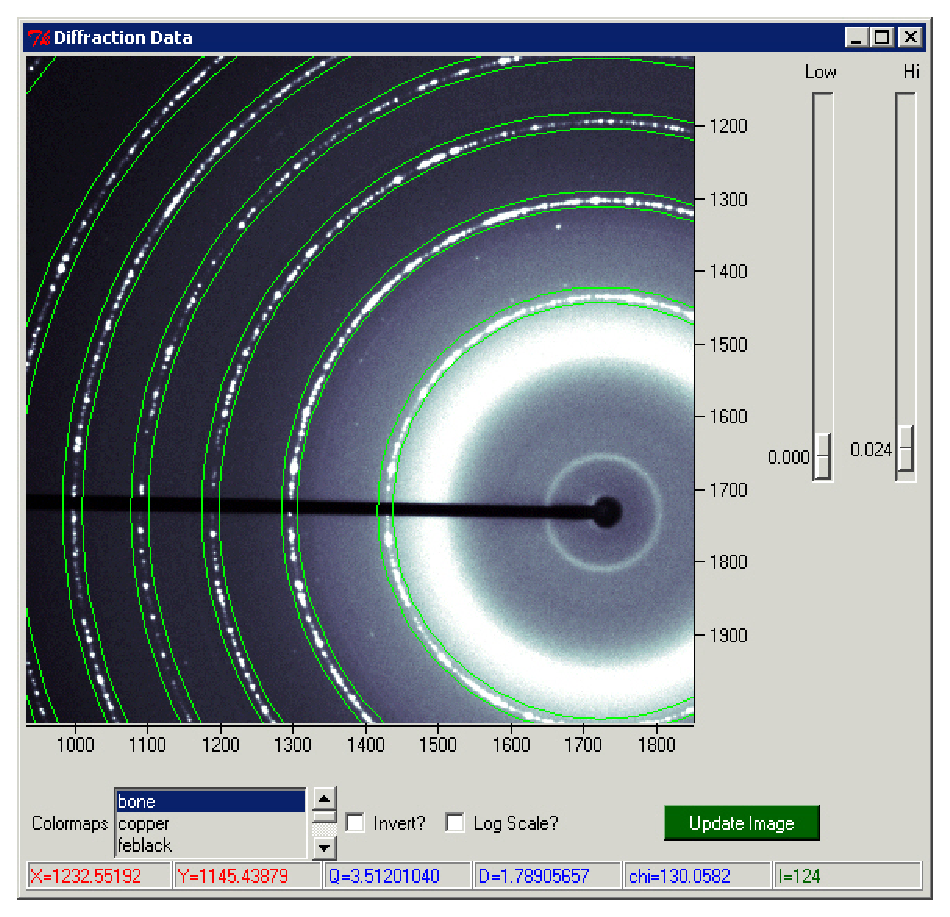
\includegraphics[scale=.75]{figures/constant_dq_lines_on_diffraction_image.eps}
    \caption{A division of a diffraction image into
    $Q$ ranges where each diffraction peak falls 
    uniquely inside one $Q$ range.}
    \label{divide_up_image}
\end{SCfigure}

\begin{SCfigure}[1][htbp]
\centering
% Generated with LaTeXDraw 1.9.3
% Tue Aug 07 18:13:48 PDT 2007
% \usepackage[usenames,dvipsnames]{pstricks}
% \usepackage{epsfig}
% \usepackage{pst-grad} % For gradients
% \usepackage{pst-plot} % For axes
\scalebox{1} % Change this value to rescale the drawing.
{
\begin{pspicture}(0,-4.3)(10.681875,4.3)
\pscircle[linewidth=0.04,dimen=outer](4.3,0.0){1.3}
\pscircle[linewidth=0.04,dimen=outer](4.3,0.0){4.3}
\psline[linewidth=0.04cm](4.4,0.1)(9.4,3.3)
\usefont{T1}{ptm}{m}{n}
\rput(8.548282,4.09){Constant $\chi$ Slice}
\psline[linewidth=0.04cm](4.36,0.48)(4.58,0.02)
\psline[linewidth=0.04cm](5.78,1.38)(6.0,0.92)
\usefont{T1}{ptm}{m}{n}
\rput(6.0514064,0.17){$Q_1$}
\usefont{T1}{ptm}{m}{n}
\rput(4.751406,-0.25){$Q_1-dQ_1$}
\psline[linewidth=0.04cm](7.0,2.12)(7.22,1.66)
\psline[linewidth=0.04cm](8.4,2.96)(8.62,2.5)
\usefont{T1}{ptm}{m}{n}
\rput(6.791406,0.71){$Q_1+dQ_1$}
\usefont{T1}{ptm}{m}{n}
\rput(8.471406,2.05){$Q_2$}
\usefont{T1}{ptm}{m}{n}
\rput(7.751406,1.31){$Q_2-dQ_2$}
\usefont{T1}{ptm}{m}{n}
\rput(9.651406,2.53){$Q_2+dQ_2$}
\psline[linewidth=0.04cm](5.16,0.88)(5.38,0.42)
\psline[linewidth=0.04cm](7.84,2.6)(8.06,2.14)
\pscustom[linewidth=0.04]
{
\newpath
\moveto(4.46,0.3)
\lineto(4.52,0.32)
\curveto(4.55,0.33)(4.6,0.365)(4.62,0.39)
\curveto(4.64,0.415)(4.675,0.45)(4.69,0.46)
\curveto(4.705,0.47)(4.73,0.5)(4.74,0.52)
\curveto(4.75,0.54)(4.775,0.59)(4.79,0.62)
\curveto(4.805,0.65)(4.82,0.715)(4.82,0.75)
\curveto(4.82,0.785)(4.82,0.86)(4.82,0.9)
\curveto(4.82,0.94)(4.835,1.02)(4.85,1.06)
\curveto(4.865,1.1)(4.905,1.16)(4.93,1.18)
\curveto(4.955,1.2)(5.015,1.22)(5.05,1.22)
\curveto(5.085,1.22)(5.16,1.205)(5.2,1.19)
\curveto(5.24,1.175)(5.305,1.15)(5.33,1.14)
\curveto(5.355,1.13)(5.395,1.105)(5.41,1.09)
\curveto(5.425,1.075)(5.455,1.05)(5.47,1.04)
\curveto(5.485,1.03)(5.53,1.02)(5.56,1.02)
\curveto(5.59,1.02)(5.64,1.04)(5.66,1.06)
\curveto(5.68,1.08)(5.73,1.11)(5.76,1.12)
\curveto(5.79,1.13)(5.83,1.15)(5.86,1.18)
}
\pscustom[linewidth=0.04]
{
\newpath
\moveto(7.08,1.92)
\lineto(7.14,1.94)
\curveto(7.17,1.95)(7.22,1.985)(7.24,2.01)
\curveto(7.26,2.035)(7.295,2.07)(7.31,2.08)
\curveto(7.325,2.09)(7.35,2.12)(7.36,2.14)
\curveto(7.37,2.16)(7.395,2.21)(7.41,2.24)
\curveto(7.425,2.27)(7.44,2.335)(7.44,2.37)
\curveto(7.44,2.405)(7.44,2.48)(7.44,2.52)
\curveto(7.44,2.56)(7.455,2.64)(7.47,2.68)
\curveto(7.485,2.72)(7.525,2.78)(7.55,2.8)
\curveto(7.575,2.82)(7.635,2.84)(7.67,2.84)
\curveto(7.705,2.84)(7.78,2.825)(7.82,2.81)
\curveto(7.86,2.795)(7.925,2.77)(7.95,2.76)
\curveto(7.975,2.75)(8.015,2.725)(8.03,2.71)
\curveto(8.045,2.695)(8.075,2.67)(8.09,2.66)
\curveto(8.105,2.65)(8.15,2.64)(8.18,2.64)
\curveto(8.21,2.64)(8.26,2.66)(8.28,2.68)
\curveto(8.3,2.7)(8.35,2.73)(8.38,2.74)
\curveto(8.41,2.75)(8.45,2.77)(8.48,2.8)
}
\end{pspicture} 
}


\caption{Here is a diagram of the peak finding algorithm. 
The solid circular black lines represent diffraction
peaks on the image. The dotted lines represent the
$Q$ ranges used to find the peaks. The diffraction
peaks are entirely within the ranges. Finally, the radial
line represents the program picking a particular $\chi$
value and looking for peaks inside of the $Q$ ranges.
Finally, the Gaussian peaks represent the program fitting
a gausian to the intensity profile inside of each of the
ranges.}
\label{fitting}
\end{SCfigure}

Our algorithm first requires\index{Peak Finding}
finding $(x,y)$ coordinates 
of many diffraction peaks. To do so, the algorithm will 
pick some $\chi$ value and then 
spread radially out from the center of the diffraction
image in this $\chi$ direction.\footnote{Remember
that the center is specified by the initial calibration 
values}. Between the given $Q$ range (for each of the $Q$ 
ranges), the program stores an array of all the data point 
on the line. It then fits a Gaussian to the data and the
$(x,y)$ coordinate of the center of this Gaussian $(x,y)$ 
is taken to be the peak. A diagram showing this algorithm
is shown in figure~\ref{fitting}. This method is
then done for many different evenly spaced $\chi$ values
and the particular value can be selected by the user
for increased accuracy.

The only really tricky part about this step is that
there is not always a consistent diffraction ring 
around the image and therefore some of these fits 
should not find peaks. Whenever this occurs, the program
just ignores the current fit and moves to the next. 
But figuring out when some particular peak is bad
is not particularly obvious. The method that this
program uses is to ensure each peak passes a few
tests. The first test is that the fit peak was
too close to the edge of the image. So any peak where
the Gaussian fit's center plus or minus twice the fit's
standard deviation gets outside of the $Q$ range is
considered too close to the edge of the image.
The next test that is done is to calculate is the
standard deviation of the data outside of the peak is
significant when compared to the height of the peak
fit. To do this, the code calculates the standard 
deviation of all the pixels that are farther then twice
the peak's fit standard deviation away from the
center of the peak. If the height of the peak
divided by this calculated background standard deviation
is smaller then some particular value, the peak is
considered bad. This value is called by the program
\gui{Stddev} and can be specified by the user from user.
\index{Stddev}
Presumably, the higher that \gui{Stddev} is, the
more picky the program is about what a good peak looks
like. This isn't the most robust method for finding peaks,
but it seems to work pretty well and it should be easy 
in principle to add new tests to the algorithm.

After compiling a list of diffraction peaks in the image,
the program can then define a residual function which
we can minimize to find the best fit calibration values.
To do so, we can convert the $(x,y)$ coordinate
of each of the peaks into a 
$(Q_{\text{peak}},\chi_{\text{peak}})$ pair. 
For each of these $(x,y)$ coordinates, we also
know what the input $Q$ list says the experimental $Q$ 
value for this peak should be (which we will call 
$Q_{\text{exp}}$). We can therefore define
the residual function as
\begin{equation}\label{residual}
    \text{Residual}(x_c,y_c,d,\lambda,\alpha,\beta,R) =  
        \sum_{\text{$x,y$ pairs}}
        (Q_{\text{peak}} - Q_{\text{exp}})^2
\end{equation}
The functional dependence comes from
calculating $Q_{\text{peak}}$ from a known
$(x,y)$ coordinate. We see that the smaller the 
Residual is, the closer we have come to finding 
the real calibration values which characterized
the diffraction experiment. If we had perfect
calibration parameters, the residual should be
equal to zero. But it is well defined for any
calibration parameters. So we can take this 
function of 7 variables and minimize it. 
The value of this function at its minimized 
is the best guess calibration values.
There are plenty of computer algorithm that
can minimize arbitrary multi-variable functions.
The one that this code uses is called the 
Levenberg-Marquardt\index{Least Squares Minimization}
nonlinear least squares algorithm
and the particular implementation that is used
to to perform the calibration is Manolis Lourakis's
levmar library\cite{lourakis04LM}. Ideally, 
once the minimization is done, a good guess at the
calibration values is found.

\section{Calibrating With the Program}

Diffraction image calibration is done with the
calibration tab of the program. This tab is shown 
in figure \ref{calibration_tab} on tab
\pageref{calibration_tab}.

As described above, to calibrate an image
you must have already loaded into the program
a diffraction data file, a $Q$ data 
file for the particular sample that was
taken, and an initial guess at the calibration 
data.

Once you have done these three things, you can
simply push the \gui{Do Fit} button to
calibrate the diffraction data. The program will
then perform the calibration algorithm as described
in section~\ref{cal_algorithm}. Once the program
finds a best guess for the new calibration
values, it will put those values into the inputs. 

While fitting the program will print to the
console some useful things. Most interesting,
the program will calculate the residual function
divided by the number of \ref{residual} and display
print the value to the terminal before and after
the calibration is done\footnote{Actually, the program
calculates the residual function divided by the number
of peaks. So it really displays the residual per peak, 
which is a more useful quantity because it would not
change if more peaks were used in the fit}
The output will look like
\begin{lstlisting}[caption={Displaying the Residual}]
 - Before fitting, the calculated residual is 5.336138e-04
 - Doing the fitting
 - After fitting, the calculated residual is 6.532131e-06
\end{lstlisting}
The program will then display the reason why the fitting
algorithm decided to quit doing the fitting and decided
that it found its best guess. For example, the program
might print out
\begin{lstlisting}[caption={Reason For Quitting}]
 - Reason for quitting the fit: 2-stopped by small gradient J^T e
\end{lstlisting}
The different reasons are told to me by the levmar fitting algorithm.
I am taking them directly from the levmar website
\url{http://www.ics.forth.gr/~lourakis/levmar/}
That website says that the different reasons why the
fitting can stop are:
\begin{itemize}
    \item stopped by small gradient J\verb!^!T e
    \item stopped by small Dp
    \item stopped by itmax
    \item start from current p with increased $\backslash$mu
    \item no further error reduction is possible. Restart with increased mu
    \item stopped by small $||$e$||$\_2\cite{lourakis04LM}
\end{itemize}
I think that the first reason to quit (stopped by smallw
gradient) means that the program found its way
to the bottom of the hill and is convinced that it did its best
job minimizing the function. I think that (stopped by itmax)
means that the program was forced to quit by a hard coded limit
to the number of loops through the fitting. So if you come across this
message, you should probably do the fit again with the current values.
I honestly don't know enough about the levmar fitting algorithm to
know what the other messages really mean. If you need to know, you 
should go into the fitting algorithm's documentation and see what you 
can find out.

The fitting algorithm also provides a covariance matrix that it finds
while fitting. I do now know how it calculates this matrix or what
it exactly what it means physically. Nevertheless, I print it out after the
fitting is done. 
\begin{lstlisting}[caption={Display of A Covariance Matrix},
    basicstyle=\ttfamily\footnotesize]
Covariance Matrix
[[  9.43e-04 -1.53e-04  5.36e-05  3.27e-03 -1.77e-03  3.64e-03  2.10e+00]
 [ -1.53e-04  1.17e-03 -1.40e-04 -8.58e-03  3.91e-05 -2.02e-04 -1.25e-01]
 [  5.36e-05 -1.40e-04  2.07e-04  1.38e-02 -1.45e-04  3.12e-04  1.78e-01]
 [  3.27e-03 -8.58e-03  1.38e-02  9.49e-01 -6.44e-03  1.40e-02  8.02e+00]
 [ -1.77e-03  3.91e-05 -1.45e-04 -6.44e-03  4.01e-01 -8.42e-01 -4.76e+02]
 [  3.64e-03 -2.02e-04  3.12e-04  1.40e-02 -8.42e-01  1.77e+00  9.99e+02]
 [  2.10e+00 -1.25e-01  1.78e-01  8.02e+00 -4.76e+02  9.99e+02  5.65e+05]]
\end{lstlisting}
The rows (from top to bottom) correspond to \gui{xc}, \gui{yc}, \gui{d}
\gui{E}, \gui{alpha}, \gui{beta}, and \gui{rotation}. The columns
(from left to right) also correspond to \gui{xc}, \gui{yc}, \gui{d}
\gui{E}, \gui{alpha}, \gui{beta}, and \gui{rotation}. I think that the
square root of the diagonal elements of the covariance matrix are supposed to 
correspond to uncertainties, but I do not know enough about the minimization
algorithm to be really comfortable saying that these are the true uncertainties in
the fit parameters. Your mileage my vary. Anyway, I print out the root of the 
diagonals. The printout by the program  
\begin{lstlisting}[caption={Display of the root of the diagonals}]
Root of the diagonal of the covariance matrix ... 
xc:  0.0307145820046
yc:  0.0341970790239
d:  0.0143735880013
E:  0.97393322373
alpha:  0.633295666676
beta:  1.32940880588
rotation:  751.595873785
\end{lstlisting}
    
If you do not like the guess for the calibration 
parameters, you can always unto to the previous
calibration values before the fit using the
\gui{Previous Values} input.

\section{\texorpdfstring{The \gui{Number of Chi?} 
        and \gui{Stddev?} Input}{The Number of 
        Chi and Stddev Inputs}}

The calibration algorithm requires starting
at the center and moving across the image in constant
$\chi$ slices (see section~\ref{cal_algorithm} or 
figure~\ref{fitting} for a graphical representation).
The number of these slices around the image that
should be done is user selectable using the 
\gui{Number Of Chi?} input. The default value is 360.
The more $\chi$ slices that are used, the slower
the fit will be.

Section \ref{fitting_sec} describes how the program
uses a parameter to determine how picky it should
be in allowing peaks that it finds. Roughly, this
parameter corresponds to how many times larger
the peak has to be then the background noise outside
of the peak. This parameter can be set using the 
\gui{Stddev?} input. The default value is 5. The higher 
the value, the less likely the program will be to find
and use bad peaks but the more likely it will be to
ignore valid good peaks.

\section{\texorpdfstring{Work in 
    $\lambda$}{Work in Lambda}}
    \label{workWavelength}

Often times, one wishes to deal with the wavelength 
of the incoming beam of light instead of the energy
of the beam. Of course, the energy and wavelength
are intemately related by the formula
\begin{equation}
    E=hc/\lambda
\end{equation}
If you wish to work with wavelength in units of
nanometers instead of energy in units of electron 
volts, you can change the state of the program so 
that the program works with wavelength instead
of energy. To do so, you have to go into the menu bar
and change the radio select from \gui{Work in eV}
to \gui{Work in Lambda}. Once you do that, the 
calibration parameter input will be labeled
$\lambda$. Any number in that input will then be converted.
After the parameter is modified during a fit,
the program will put the wavelength value into
the input. Finally, when the calibration
parameters are saved to a file, the wavelength will
saved to the file instead of the energy.


\section{Fixing Calibration Parameters}
\label{fix_parameters}

When fitting calibration parameters, it is not
always desirable to allow the program to vary
all of the calibration parameters. For example,
the energy of the beam used during the diffraction
experiment might be already very well known already
so there would be no reason to calibrate the energy.
If you wish to fix any of the calibration parameters
values so that it does not vary during a calibration
fit, you can use the check boxes under the \gui{Fixed?}
label to fix the parameter. When the corresponding
check box is checked, the parameter will not vary
during the fit. When it is not checked, the
parameter will vary during the fit. You
can not fix the pixel length and 
pixel height because they are always held fixed. This is 
because these are never
the short of thing that one would want to vary.
They are some property of the detector that is known in
advance.

\section{\texorpdfstring{Displaying Constant $Q$ 
    Lines}{Displaying Constant Q Lines}}
    \label{displayconstQlines}

After the program has been given a diffraction file,
a list of the constant $Q$ lines, and some
calibration parameters, the program has a very
useful feature where it can display on top of
the image the diffraction pattern that should
show up for the particular $Q$ lines and the
particular calibration parameters.

The \gui{Draw Q Lines?} button on the 
\gui{Calibration} tab enables this.
Figure~\ref{constant_q_lines_on_diffraction_image}
shows what the diffraction image looks like with
the $Q$ lines drawn on it.

\begin{SCfigure}[1][htbp]
    \centering
    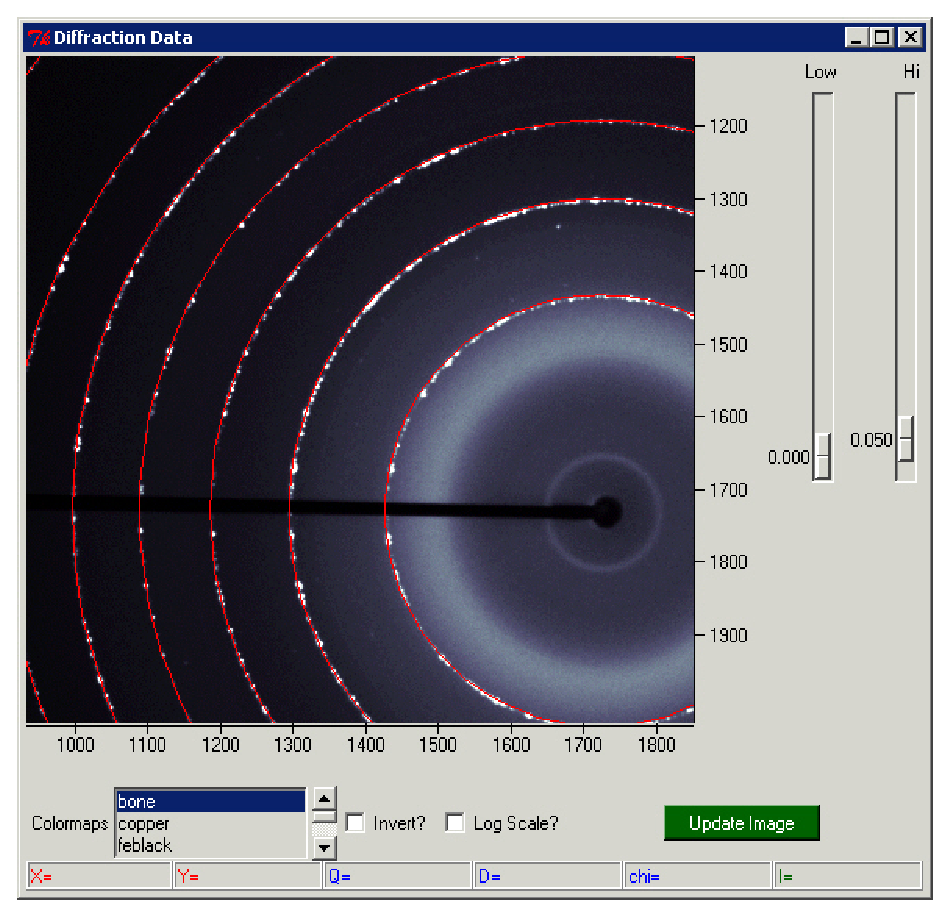
\includegraphics[scale=.75]{figures/constant_q_lines_on_diffraction_image.eps}
    \caption{A diffraction image with constant the 
    $Q$ lines displayed on it.}
    \label{constant_q_lines_on_diffraction_image}
\end{SCfigure}

Drawing these lines is actually very easy. For
each $Q$ value, the program picks a lot of
$\chi$ values. We know that each of the $Q$, $\chi$
values is in the constant $Q$ line so we can use
the calibration parameters to convert them to $x$, $y$
values and connect all the pixel coordinates to 
make the line.

Constant $Q$ lines can also be drawn on top of the
caked data. This is described in 
section~\ref{cakeQlinesandpeaks}.  
The color of the $Q$ lines can be changed using the
\gui{Color} button next to the \gui{Draw Q Lines?} 
button.

\section{\texorpdfstring{Displaying Constant $\Delta Q$ 
        Lines}{Displaying Constant delta Q Lines}}
        \label{displayconstdQlines}
        

The program needs in addition to the $Q$ values
a range in $Q$ to find the peaks. See 
section~\ref{fitting_sec} for more details. Because
the program has this range, it can also display the
$\Delta Q$ range on top of the image.
This can be done with the \gui{Draw dQ Lines?} button
and the color of these lines can be changed with the
corresponding \gui{Color} button. 
Figure~\ref{constant_dq_lines_on_diffraction_image}
shows what the diffraction image looks like with
the $\Delta Q$ lines drawn on it.

\begin{SCfigure}[1][htbp]
    \centering
    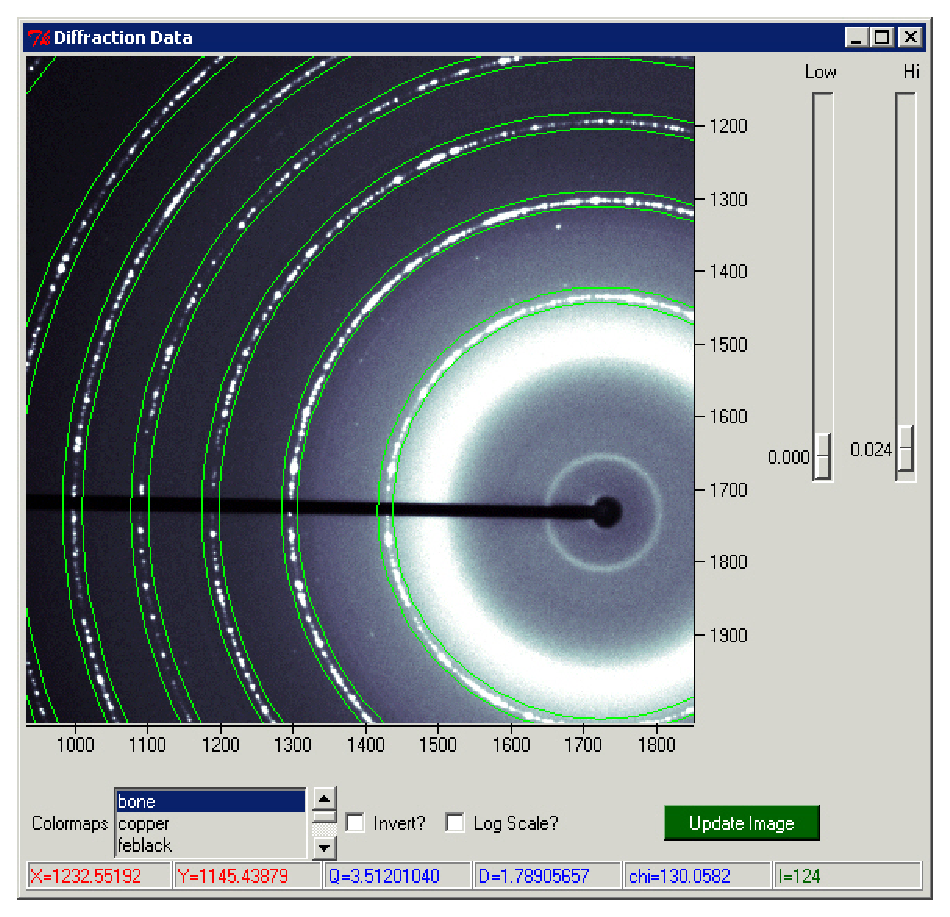
\includegraphics[scale=.75]{figures/constant_dq_lines_on_diffraction_image.eps}
    \caption{A diffraction image with the constant 
    $\Delta Q$ lines displayed upon it.}
    \label{constant_dq_lines_on_diffraction_image}
\end{SCfigure}


Constant $\Delta Q$ 
lines can also be drawn on top of the caked data. This 
is described in section~\ref{cakeQlinesandpeaks}.

\section{Displaying Peaks}\label{displaying_peaks_diffraction}

Section~\ref{fitting_sec} describes how the program has to find a bunch
of peaks on the diffraction image in order to perform the calibration.
After the program has found all the peaks, it can conveniently display
them on top of the diffraction image. This can be done with the
\gui{Draw Peaks?}. The peaks will be displayed as crosses and the color
of the peaks can be changed with the corresponding \gui{Color} button.
Figure~\ref{peaks_on_diffraction_image} shows what the diffraction image
looks like with the peaks drawn on it. This feature is useful because 
you can use it to see if the program is actually finding real peaks
corresponding to diffraction maxima. If many of the peaks that the program 
finds do not correspond to diffraction maxima, it is less likely that 
the program would do a good job calibrating the diffraction image.

\begin{SCfigure}[1][htbp]
    \centering
    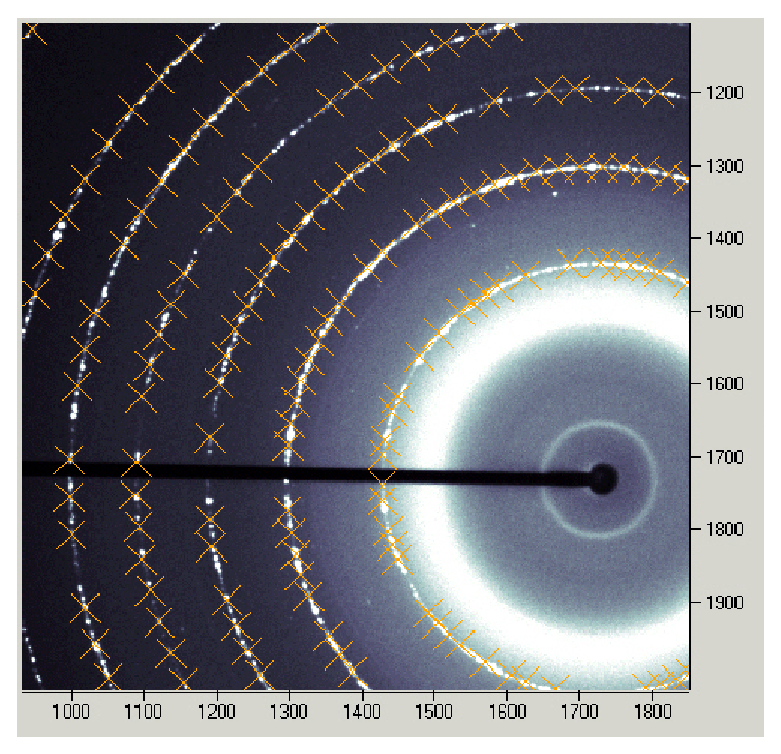
\includegraphics[scale=.75]{figures/peaks_on_diffraction_image.eps}
    \caption{A diffraction image with the peaks displayed upon it.}
    \label{peaks_on_diffraction_image}
\end{SCfigure}

Peaks can also be drawn on top of the caked data. This 
is described in section~\ref{cakeQlinesandpeaks}.

\section{Masking Peaks}

\begin{figure}[htb]
    \centering
    \subfloat[A diffraction image with diffraction peaks
    and two polygon masks displayed on top of it.]{
    \label{mask_peaks_diffraction}
    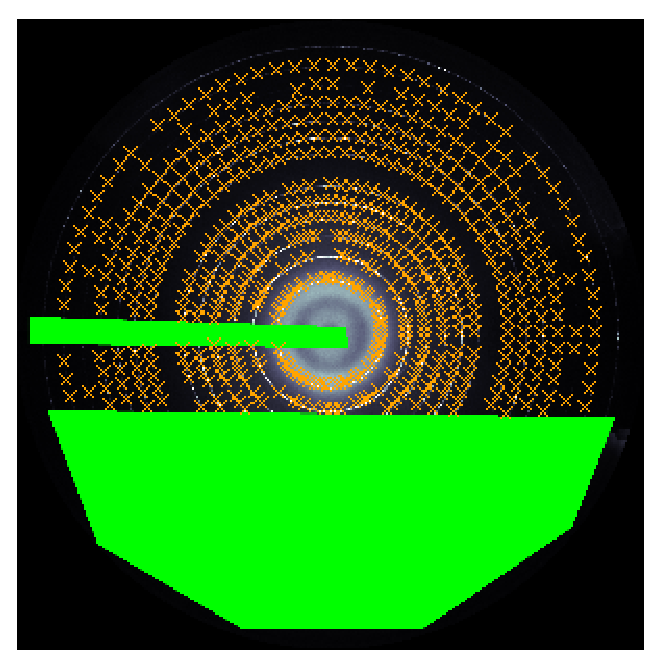
\includegraphics[scale=.75]{figures/mask_peaks_diffraction.eps}}
    \subfloat[A caked plot with diffraciton peaks and
    two polygon masks displayed on top of it.]{
    \label{mask_peaks_cake}
    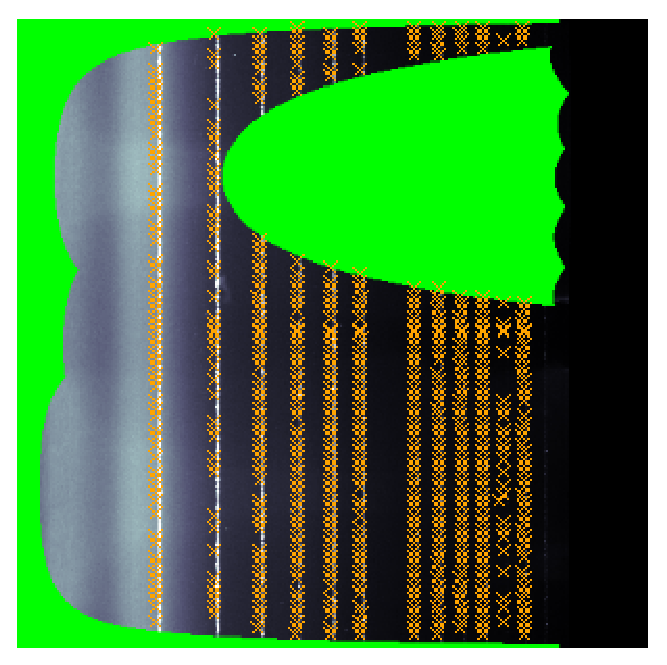
\includegraphics[scale=.75]{figures/mask_peaks_cake.eps}}		
    \caption{Polygon masks can be used to block
    out certain regions of the image. Whenever
    a polygon mask is loaded into an image, none
    of the peaks found in the mask's region will be
    used while calibrating the image. Furthermore,
    none of the peaks within the masks will be 
    displayed on the diffraction image or caked plot.}
    \label{mask_peaks}
\end{figure}

The general idea behind masking peaks is allow polygon 
masks (see chapter~\ref{pixel_masking}) to be used as 
a way to forbit the program from using any peaks found
within a certain region. So if a polygon mask covers a 
certain area of the image, none of the peaks found within that
area will be used while calibrating. Also, none of 
the peaks will be displayed on top of the diffraction 
image or cake image. An example of this is shown in
figure~\ref{mask_peaks_diffraction}. 
See section~\ref{displaying_peaks_diffraction}
for a discussion of displaying peaks on a diffraction
image.  Figure~\ref{mask_peaks_cake} shows the same effect 
on top of the corresponding caked plot. See 
chapter~\ref{Caking} for a discussion of caking.
In particular, see section~\ref{displaying_peaks_cake} 
for more information on displaying peaks on a caked
image. This feature was added in version 2.0.0.

\section{Saving the Peak List}

The program has a feature where it can generate
a list of diffraction peaks that it finds the 
diffraction image (just like when it is calibrating)
but then instead of calibrating the image, the program
saves out all of the peaks to a data file. This can
be useful, for example, if you need a list of pixel 
coordiantes where diffraction peaks are for some further
data analysis. The \gui{Make/Save Peak List} button can
be used to save out the peak list. Just as in calibrating,
the program requires in advance for a diffraction file to
be loaded, for a standard $Q$ file to be loaded, and for
a guess at the calibration parameters to be in the inputs.

A typical peak list file looks like\footnote{I have modified
what a real file looks like a bit. The numbers are really tab 
separated but I show them space separated for brevity.}
\begin{lstlisting}[caption={A Peak List File,basicstyle=\ttfamily\tiny}]
# A list of peaks found in the diffraction image.
# Calculated on Sun Apr  6 18:06:56 2008
# Calibration data used to find peaks:
#   x center:    1725.0000000 pixels
#   y center:    1725.0000000 pixels
#   distance:     122.5040000 mm
#   energy:     12714.2388941 eV
#   alpha:          0.0000000 degrees
#   beta:           0.0000000 degrees
#   rotation:       0.0000000 degrees
#   pixel length:     100.0000000 microns
#   pixel height:     100.0000000 microns
#   x  y  RealQ  FitQ  chi  width  intensity  2theta
2016.15  1724.44  1.511  1.50  0.11  0.0075 5564.32  13.36
2016.68  1719.33  1.51  1.50  1.11  0.0093 1662.72  13.39
\end{lstlisting}
First, the file contains the calibration parameters
used to generate the peaks. Then it has a comment string
describing each of the numbers in each of the rows
that follow. Each row corresponds to a unique peak.
The first two numbers $x$ and $y$ are
the $x$ and $y$ pixel coordinate corresponding to
a location in the diffraction image of the peak. RealQ 
is the $Q$ value found in the $Q$ list that is already 
known. FitQ is the $Q$ value calculated 
from the $(x,y)$ coordinate using the calibration
parameters. $\chi$ is also calculated from the pixel
coordinate using the calibration parameters. 
Intensity is intensity value found in the data at
this peak. $2\theta$ is calculated at the $(x,y)$ 
coordinate using the calibration parameters.

\section{Handling Calibration Data}

There are inputs in the calibration tab of the
program for input of the calibration parameters.
\gui{xc} is for the $x$ center, \gui{yc} is
for the y center, \gui{d} is for the distance,
\gui{E} (or \gui{$\lambda$:}) is for the energy
or wavelength. The $\alpha$, $\beta$, and
$R$ inputs are for the three angles. 
\gui{pl} stands for the pixel length
and \gui{ph} stands for the pixel height.

You can directly input calibration data using 
the inputs and once the data is in the inputs
it can be used by the program to do the calibration
(or the caking or anything else).

But there are a couple of other ways to deal
with calibration data.
You can load and save calibration program
from the program using the \gui{Load From File}
and \gui{Save To File} buttons. This is nice
because it can be used, for example, to save 
the data that was found by calibration data
for future reference. As you will see, the 
calibration data files can handle information
about whether the parameters should be fixed
(see section \ref{fix_parameters}).

The format for a calibration data file is 
pretty simple. Below is  an example
\begin{lstlisting}[caption={Calibration Parameters}]
# Calibration File
xc	1725.000000	0
yc	1725.000000	0
D	125.296000	0
E	12735.395772	0
alpha	0.000000	0
beta	0.000000	0
rotation	0.000000	0
pixelLength	100.000000
pixelHeight	100.000000
\end{lstlisting}
Comment lines beginning with
a \# and are ignored. Each of the parameters
gets its own line. Each parameter name is 
followed by some spaces or tabs and then the
value. The value can be followed by an optional
second number which is either zero or one.
The second number corresponds to whether or
not the parameter should be fixed while
fitting. One means fix the parameter. Zero means
let it very. If no number is given, the default
is to not fix the parameter.

Instead of energy, the wavelength of the incoming
beam of light can be stored in a calibration file.
The wavelength line would look like 
\macroline{wavelength	0.973540}.
When the program is in wavelength mode, the program
will save out calibration parameters with this line
instead of the one above. The program will load in a 
file containing either no matter what mode the program 
is in. It will do the conversion if it has to do put 
the right value into the input. See 
section~\ref{workWavelength}.


\section{\texorpdfstring{Handling $Q$ Data}{Handling Q Data}}
\label{TheQValues}\index{Q Data}

$Q$ data is always loaded into the program from files. 
$Q$ data can be loaded into the program with the \gui{Q Data:}
input on the calibration tab. 
You can either type in the filename of the $Q$ file by hand 
and push the load button or click on the folder icon to the 
side and use the file selector to pick the file that you want.

The $Q$ data file format is pretty simple. Below is an example 
\begin{lstlisting}[caption={Lanthanum Hexaboride.dat},label=LaB6]
# This is Q Data for Lanthanum Hexaboride
Q   dQ
1.511543809 .05
2.137646823 .05
2.618102966 .05
3.023087619 .05
3.379873753 .05
3.702525225 .05
...
\end{lstlisting}
Comment lines beginning with a \# and are always ignored. The
first line in the file should be of the form "Q  dQ" or "Q  delta Q" 
to specify that this is a list of $Q$ values. The rest of the
file should have $Q$ values followed a $\Delta Q$ range.
All $Q$ values must be larger than 0. None of the $Q$ ranges can 
overlap. Instead of inputting $Q$ values, the program can input
$D$ values if the first line is instead "D dD" or "D delta D"
The values should be given instead in $D$ space and the values
will be converted using~\ref{DtermsQ}.

\section{\texorpdfstring{The \gui{Get From Header?} Input}
    {The ''Get From Header Input''}}

Often times guesses at the experimental parameters are 
stored in the header data inside of the diffraction image. 
The program can try to find these header calibration parameters
and put them into the calibration parameters inputs in the 
program. This can be done with the \gui{Get From Header} 
button.



